% Q01(b) -- Boundary-scan architecture (IEEE 1149.1 / JTAG).
% NOTE: standard JTAG architecture (not in the course notes) -- TDI shifts through a ring
% of boundary-scan cells wrapping the core logic to TDO; a TAP controller FSM (TMS,TCK)
% and an instruction register control the boundary-scan register.
\documentclass[border=10pt]{standalone}
\usepackage{tikz}
\usetikzlibrary{arrows.meta,positioning}
\begin{document}
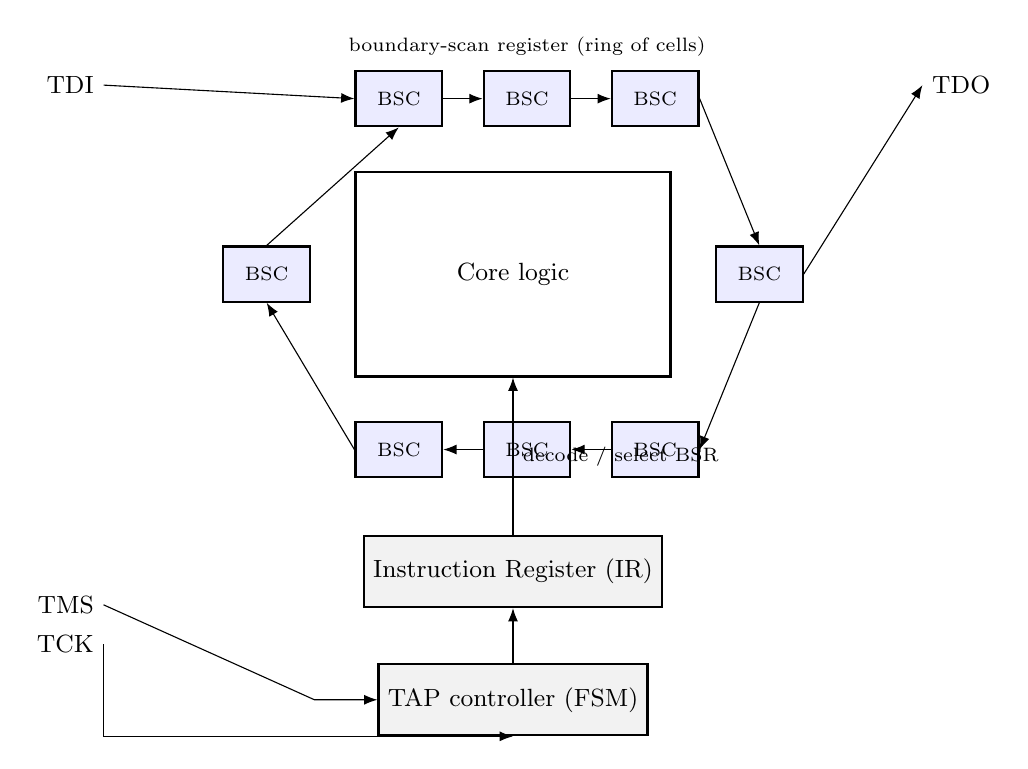
\begin{tikzpicture}[>=Latex, font=\small,
  core/.style={draw, thick, minimum width=4cm, minimum height=2.6cm, align=center},
  bsc/.style={draw, thick, fill=blue!8, minimum width=1.1cm, minimum height=0.7cm,
              font=\scriptsize, align=center},
  ctl/.style={draw, thick, fill=gray!10, minimum width=3.2cm, minimum height=0.9cm,
              align=center}]
% central core logic
\node[core] (core) {Core logic};
% boundary-scan cells forming a ring around the core
\node[bsc, above=0.55cm of core.north west, anchor=south west] (t1) {BSC};
\node[bsc, right=0.5cm of t1] (t2) {BSC};
\node[bsc, right=0.5cm of t2] (t3) {BSC};
\node[bsc, below=0.55cm of core.south west, anchor=north west] (b1) {BSC};
\node[bsc, right=0.5cm of b1] (b2) {BSC};
\node[bsc, right=0.5cm of b2] (b3) {BSC};
\node[bsc, left=0.55cm of core.west] (l1) {BSC};
\node[bsc, right=0.55cm of core.east] (r1) {BSC};
\node[align=center, above=0.05cm of t2, font=\scriptsize] {boundary-scan register (ring of cells)};
% TDI in, chain through the ring, TDO out
\draw[->] (-5.2,2.4) node[left]{TDI} -- (t1.west);
\draw[->] (t1) -- (t2); \draw[->] (t2) -- (t3);
\draw[->] (t3.east) -- (r1.north);
\draw[->] (r1.south) -- (b3.east);
\draw[->] (b3) -- (b2); \draw[->] (b2) -- (b1);
\draw[->] (b1.west) -- (l1.south);
\draw[->] (l1.north) -- (t1.south);
\draw[->] (r1.east) -- (5.2,2.4) node[right]{TDO};
% instruction register
\node[ctl, below=2.0cm of core.south] (ir) {Instruction Register (IR)};
\draw[->] (ir.north) -- (core.south) node[midway,right,font=\scriptsize]{decode / select BSR};
% TAP controller FSM
\node[ctl, below=0.7cm of ir] (tap) {TAP controller (FSM)};
\draw[->] (-5.2,-4.2) node[left]{TMS} -- ([xshift=-0.8cm]tap.west |- tap.west) -- (tap.west);
\draw[->] (-5.2,-4.7) node[left]{TCK} |- (tap.south);
\draw[->] (tap.north) -- (ir.south);
\end{tikzpicture}
\end{document}
